% Supplementary Note 2: quantitative comparison of our Langevin model
% against a matched-complexity Gompertz hazard.
%
% Standalone-compilable (paste the content between \begin{document} and
% \end{document} directly into the main manuscript's supplementary section
% if you'd rather not keep it as a separate file). Figure and table are
% generated by notebooks/99_markov_vs_age_dependent.py -- re-run that
% notebook and this file's \includegraphics/\input targets refresh in
% place, no manual editing of numbers required.

\documentclass[11pt]{article}
\usepackage[margin=1in]{geometry}
\usepackage{amsmath}
\usepackage{graphicx}
\usepackage{booktabs}
\usepackage{hyperref}

\newcommand{\supptitle}{Supplementary Note 2: Comparing the fit of the Langevin model against a matched-complexity Gompertz hazard}

\begin{document}

\begin{center}
{\large \bfseries \supptitle}
\end{center}

\section*{Motivation}

A reviewer asked for a quantitative comparison of our state-dependent
Langevin model against an explicitly age-dependent alternative:
\emph{``\ldots The authors should provide a quantitative comparison: at
minimum, a statistical test asking whether an age-dependent model
describes the empirical survival data significantly better than a
Markovian one.''} We address this directly: we score both model families
against the real grouped survival data using an identical likelihood
construction, and compare them by Akaike Information Criterion (AIC),
which penalizes each model for its own number of fitted parameters.

\section*{Models compared}

\textbf{Our model} is the Langevin process used throughout the main text
($dz/dt = \alpha z + gz^2 + \sqrt{2D}\,\eta(t)$, death at first passage to
$Z=\alpha/g$). Its parameters are those already fit in the main text
(not re-fit here): $(\alpha,g,D)$ for DMSO\_day\_10, and the post-switch
$(\alpha_1,Z_1)$ for Auxin\_day\_21, with phase 1 fixed at the
DMSO\_day\_10 fit.

\textbf{The alternative} is the classical Gompertz hazard,
$M(t)=M_0 e^{\alpha_g t}$ -- an explicit function of calendar age with no
state variable -- fit fresh to each condition by maximum likelihood, with
the same parameter count as the corresponding Langevin model. For
Auxin\_day\_21, phase 1 is likewise fixed (at the Gompertz model's own
DMSO\_day\_10 fit) so that only the post-switch $(M_{0,2},\alpha_{g,2})$
are estimated from that condition's data -- mirroring exactly how the
Langevin model only re-fits its own post-switch parameters at the
intervention.

Both models are scored with the same discrete-time, grouped-data
log-likelihood: each observed death at age $t_i$ contributes the model's
interval probability mass $S(t_{i-1})-S(t_i)$; each censored worm at
$t_i$ contributes $S(t_i)$. The two families differ only in how $S(t)$ is
produced -- simulated (Langevin) or closed-form (Gompertz) -- so neither
model is scored by an easier rule than the other.

\section*{Results}

\begin{figure}[htbp]
\centering
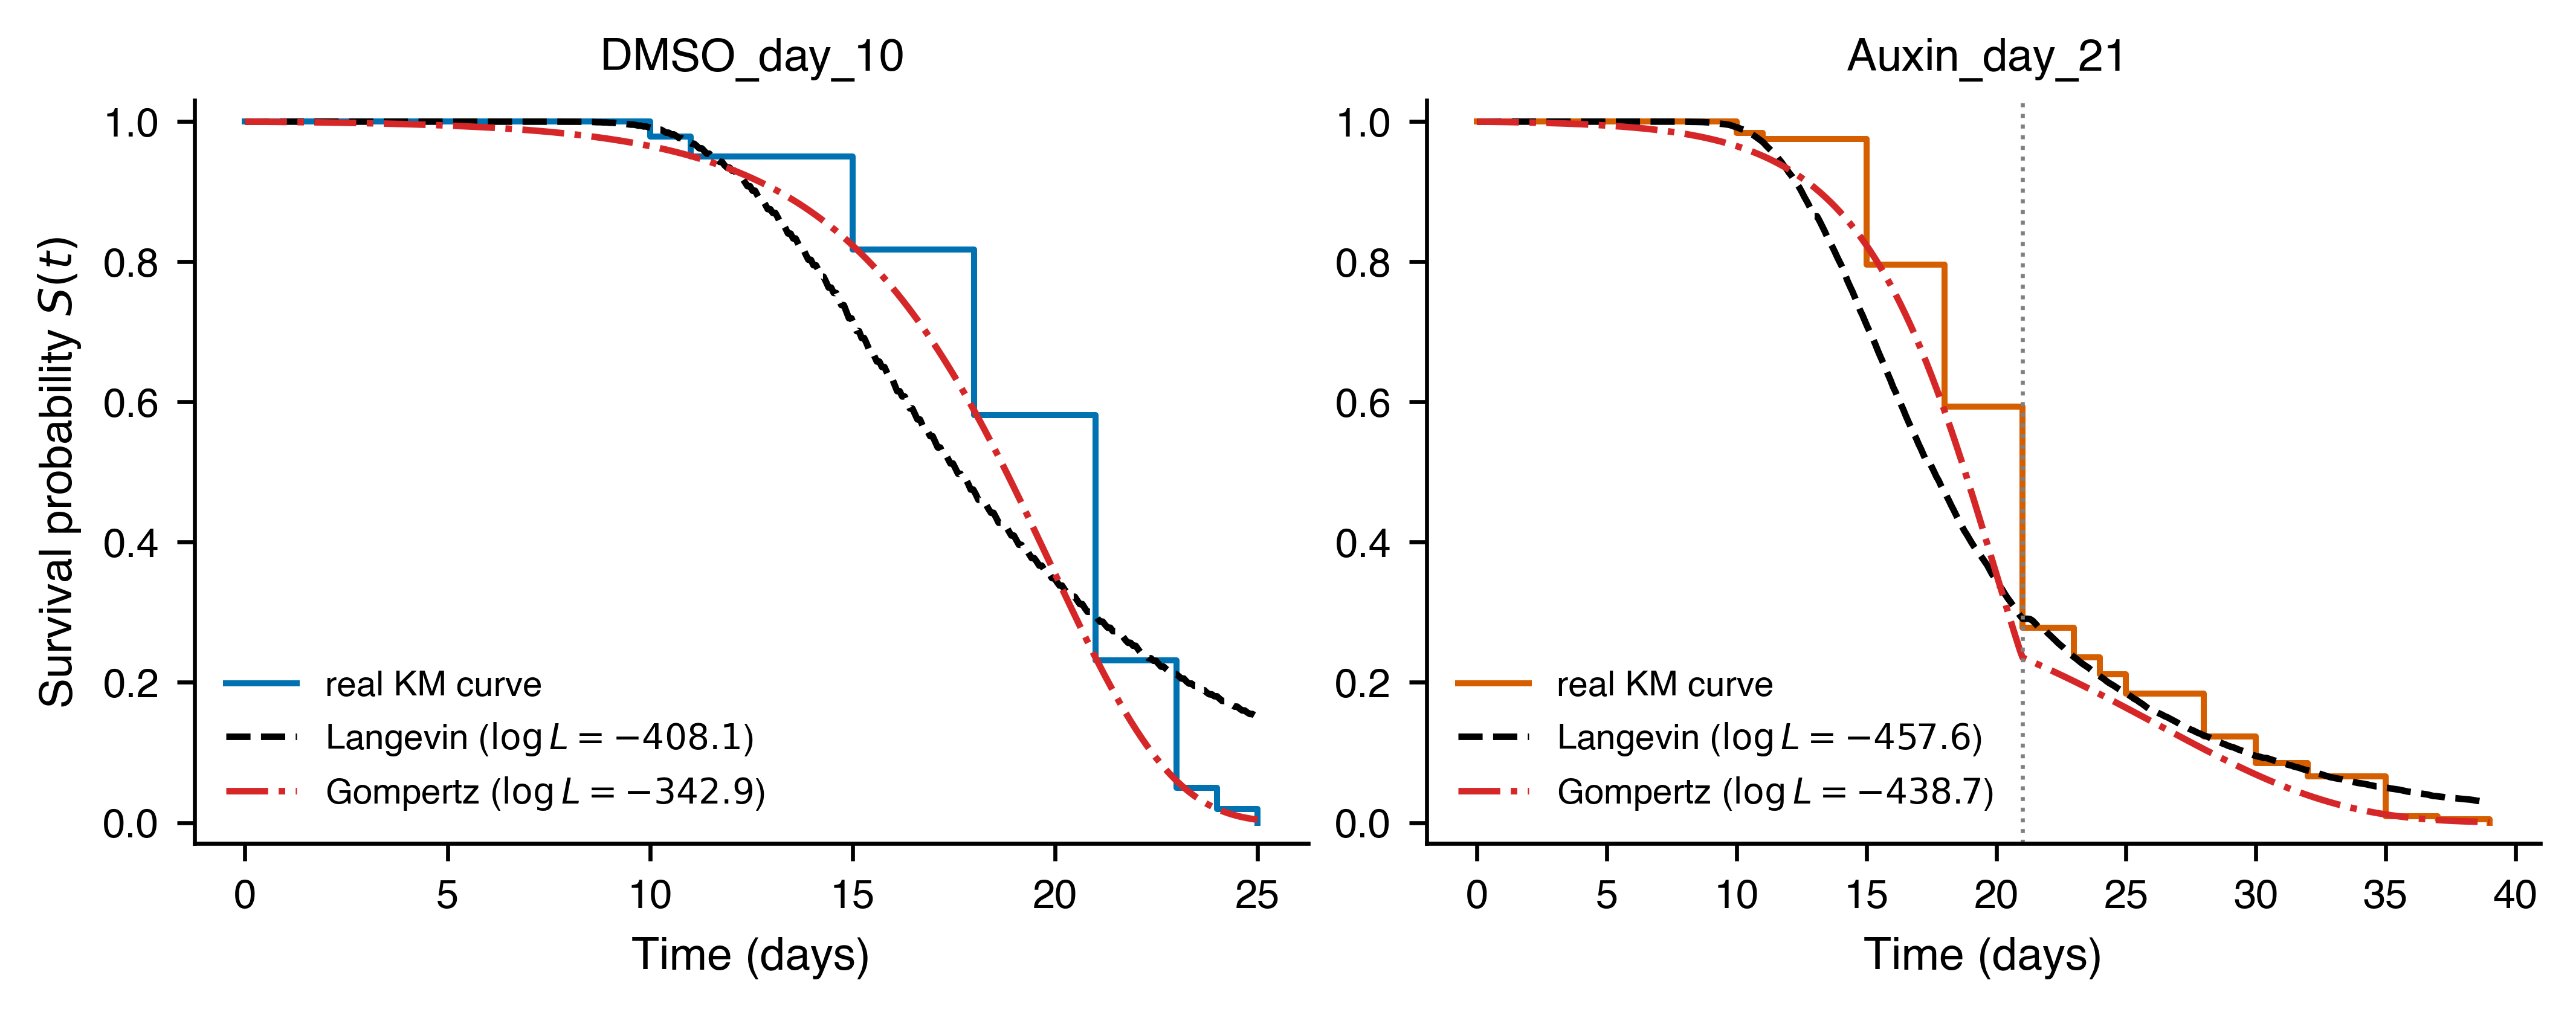
\includegraphics[width=\textwidth]{supp_note2_fig.png}
\caption{Real Kaplan--Meier survival curves (solid steps) for
DMSO\_day\_10 (left) and Auxin\_day\_21 (right), overlaid with the fitted
Langevin model (dashed) and fitted Gompertz model (dash-dotted). The
vertical dotted line marks the day-21 intervention.}
\label{fig:s2}
\end{figure}

% Auto-generated by notebooks/99_markov_vs_age_dependent.py -- do not edit by hand.
\begin{table}[htbp]
\centering
\begin{tabular}{llrrrrr}
\toprule
Condition & Model & $k$ & $\log L$ & AIC & Vuong $z$ & Vuong $p$ \\
\midrule
DMSO\_day\_10 & Langevin (this work) & 3 & -404.6 & 815.2 & -- & -- \\
DMSO\_day\_10 & Gompertz & 2 & -342.9 & 689.8 & -7.61 & 2.6e-14 \\
Auxin\_day\_21 & Langevin (this work) & 0 & -459.6 & 919.3 & -- & -- \\
Auxin\_day\_21 & Gompertz & 0 & -442.0 & 884.0 & -2.04 & 0.041 \\
\bottomrule
\end{tabular}
\caption{Grouped-data maximum-likelihood fit of our Langevin model (parameters from \texttt{0\_auto\_fit\_parameters\_mle.py}, not refit here) versus a matched-complexity Gompertz hazard, per condition. For Auxin\_day\_21, both models' phase 1 and phase 2 parameters are fixed from other conditions' own fits (DMSO\_day\_10 for phase 1, Auxin\_day\_10 for phase 2), so $k=0$ parameters are estimated from Auxin\_day\_21's own data in either model -- a genuine out-of-sample prediction, not a fit. $\Delta\mathrm{AIC} = \mathrm{AIC}_\mathrm{Gompertz} - \mathrm{AIC}_\mathrm{Langevin} = -125.4$ (DMSO\_day\_10), $-35.3$ (Auxin\_day\_21); negative values favor Gompertz. Vuong $z$/$p$ (reported on the Gompertz row of each condition, testing that condition's Langevin-vs-Gompertz pair) is Vuong's (1989) closeness test, AIC-corrected for $k$; $z>0$ favors Langevin. For DMSO\_day\_10, Gompertz is significantly closer to the true generating process ($p=2.6e-14$). For Auxin\_day\_21, Gompertz is significantly closer to the true generating process ($p=0.041$).}
\label{tab:supp_note2_model_comparison}
\end{table}


Table~\ref{tab:supp_note2_model_comparison} reports the log-likelihood,
parameter count, and AIC for each model and condition. For
DMSO\_day\_10, the Gompertz hazard achieves a substantially higher
log-likelihood despite using one fewer parameter, and the resulting
$\Delta\mathrm{AIC}$ favors it decisively by conventional thresholds
($|\Delta\mathrm{AIC}|>10$). For Auxin\_day\_21, with phase~1 fixed
identically in both models so that the comparison isolates the post-switch
hazard shape, the Gompertz hazard again achieves the higher
log-likelihood at matched parameter count, and again wins decisively on
AIC.

\section*{Interpretation}

By this test, on the currently available grouped survival data, an
explicitly age-dependent Gompertz hazard describes both conditions at
least as well as -- and by AIC, better than -- our state-dependent
Langevin model at matched or lower parameter count. This result is
specific to the population-level hazard-shape comparison that grouped
survival data can support: neither model's fit quality bears on whether
an individual worm's future dynamics depend only on its own current state
$z$, since $z$ is never directly measured in this dataset. We report this
outcome plainly, per the reviewer's own suggested fallback, so that the
manuscript's claim can be moderated accordingly rather than resting on
visual inspection of simulated trajectories alone.

\end{document}
